\documentclass[problem]{mcs}

\begin{pcomments}
  \pcomment{MQ_binary_relation_terms}
  \pcomment{Xiaoyue 9/13}
\end{pcomments}

\pkeywords{
  relation
  image
  injection
  surjection
  total
  function
  inverse
  arrow
}
%%%%%%%%%%%%%%%%%%%%%%%%%%%%%%%%%%%%%%%%%%%%%%%%%%%%%%%%%%%%%%%%%%%%%
% Problem starts here
%%%%%%%%%%%%%%%%%%%%%%%%%%%%%%%%%%%%%%%%%%%%%%%%%%%%%%%%%%%%%%%%%%%%%

\begin{problem}
Figure \ref{fig:img} shows the arrow diagram for a relation $R$.

\begin{figure}[h]

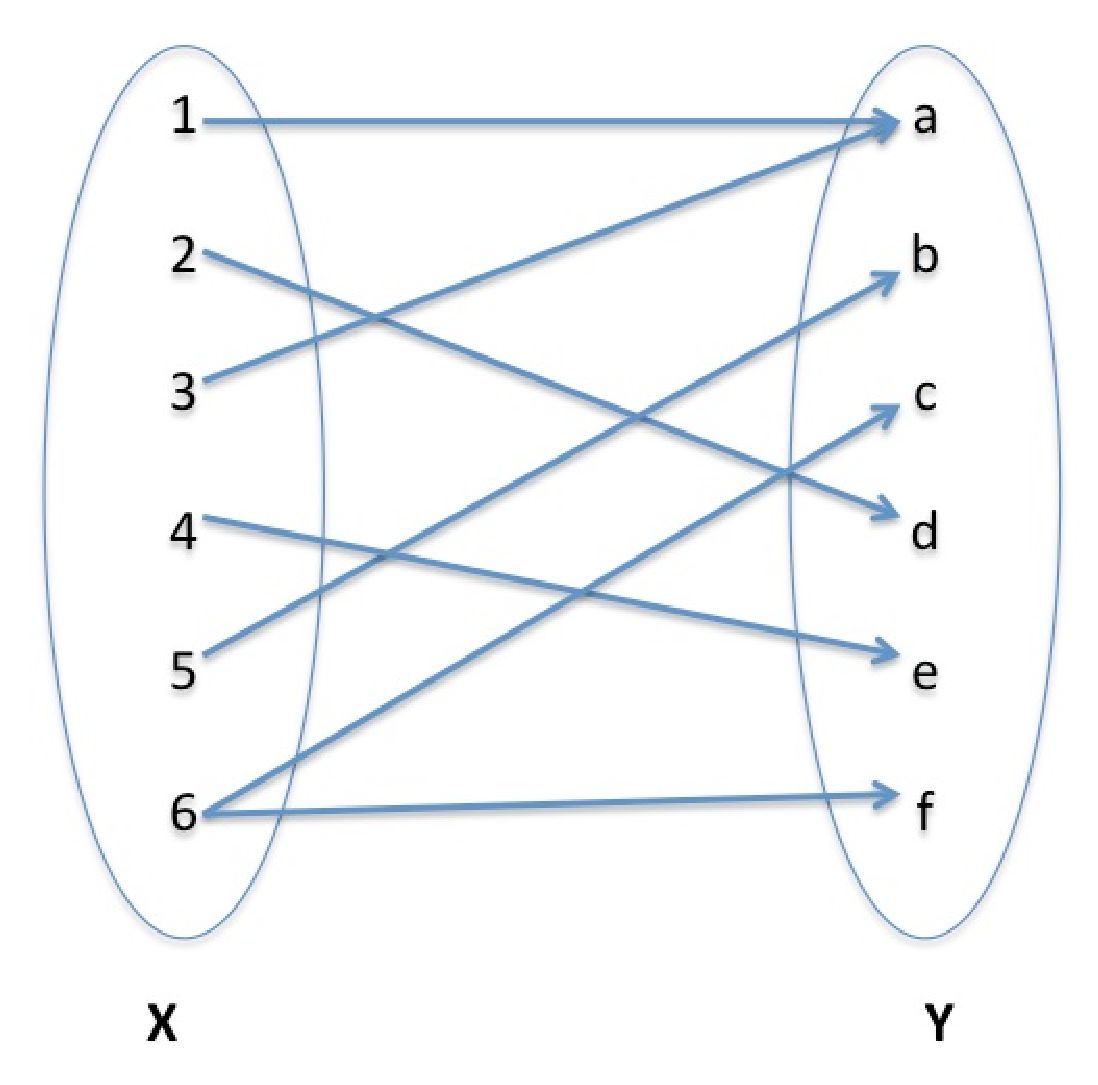
\includegraphics[height = 2in ]{image-inverseimage1}

\caption{Relation $R$.}
\label{fig:img}
\end{figure}
\bparts

\ppart What is the image under $R$ of the even numbers in domain $X$?\hfill\brule{1.5in}\label{evenimage}

\begin{solution}
\[
\set{c, d, e, f}
\]
\end{solution}


\ppart What is the inverse image under $R$ of the vowels in codomain $Y$?\hfill\brule{1.5in}\label{vowelimage}

\begin{solution}
\[
\set{1, 3, 4}
\]
\end{solution}


\inbook{
\ppart List the first letters of \emph{all} the properties below
satisfied by relation $R$.\hfill\brule{1.0in}\label{arrowprop-letters}
\begin{center}
 \textbf{f}unction [$\le 1$ out] \qquad \textbf{t}otal [$\ge 1$ out]

 \textbf{i}njective [$\le 1$ in] \qquad \textbf{s}urjective [$\ge 1$ in]
 \qquad \textbf{b}ijective [$=1$ in \& out]
\end{center}

\begin{solution}
\textbf{t}otal $[\ge 1\ \text{out}]$ and \textbf{s}urjective $[\ge 1\ \text{in}]$.
\end{solution}
}

\eparts


\end{problem}
%%%%%%%%%%%%%%%%%%%%%%%%%%%%%%%%%%%%%%%%%%%%%%%%%%%%%%%%%%%%%%%%%%%%%
% Problem ends here
%%%%%%%%%%%%%%%%%%%%%%%%%%%%%%%%%%%%%%%%%%%%%%%%%%%%%%%%%%%%%%%%%%%%%

\endinput
